\section{Architecture and Design Decisions}\label{sec:arch}
Fig.~\ref{fig:arch} shows the architecture, which follows the reference design with the substitutions listed in Table~\ref{tab:alt}.
\begin{figure}[t]\centering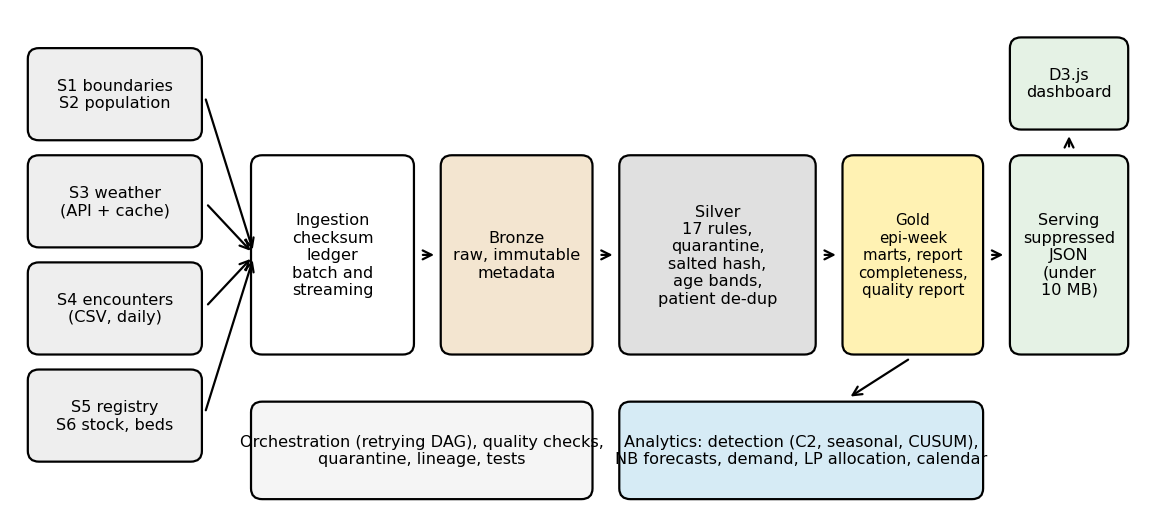
\includegraphics[width=\columnwidth]{figures/architecture.png}\caption{EpiScope architecture: sources, medallion lakehouse, analytics, suppressed serving layer and D3.js dashboard.}\label{fig:arch}\end{figure}

\textbf{Layers.} Bronze stores every landed file unmodified as strings plus \texttt{\_source}, \texttt{\_batch\_id} (first 12 hex digits of the file SHA-256), \texttt{\_file\_checksum}, \texttt{\_load\_ts}, \texttt{\_source\_file} and \texttt{\_source\_date}. Silver parses, validates against 17 rules, quarantines failures with reason codes, replaces the patient identifier by a salted SHA-256 hash, reduces age to a band, joins geography and flags cross-facility duplicate patients. Gold holds the epi-week marts: a reporting triangle (onset week by report week), weekly cases by onset week, weekly reports by report week, district report completeness, weekly weather, district stock at the end of each week, and the data-quality report. Tables are registered in the Spark SQL catalog (Hive metastore backed by Derby) under database \texttt{episcope}.

\textbf{Partitioning (ING-3).} Silver is partitioned by \texttt{epi\_year/epi\_week} of onset: almost every query is a time window, and late records (up to three weeks, longer after back-fill) touch only the most recent partitions, which can therefore be replaced with dynamic partition overwrite. Division was rejected as a partition key because eight divisions times 262 weeks would create about 2000 partitions of a few thousand rows each (the small-file problem); district is instead a column used for filtering, benefiting from Parquet min/max statistics. Gold marts use the same key. The epi-week is defined by weeks starting on Sunday and belonging to the year of their Wednesday.

\textbf{Incremental, idempotent loads (ING-4).} A ledger of file checksums makes bronze ingestion a no-op for files already loaded. Silver processes only bronze batches missing from its own ledger, computes the affected epi-weeks (plus one week either side, because a patient duplicate can straddle a week boundary), reads those existing partitions, merges, and rewrites exactly those partitions through a staging directory (Spark refuses to overwrite a path it is reading). Gold rebuilds only the weeks that silver reports as changed. A record resubmitted in a later file is rejected with reason R17 and never alters counts. An integration test loads a two-month history, re-runs it, then lands a file with three late records and one resubmission and asserts exact count changes in one epi-week.

\begin{table}[t]\caption{Design alternatives considered.}\label{tab:alt}\centering\small
\begin{tabularx}{\columnwidth}{@{}lXX@{}}\toprule
Decision & Chosen & Alternatives and reason \\\midrule
Table format & Parquet, ledger-based merge & Delta/Iceberg~\cite{delta}: time travel is attractive but adds a dependency; the reporting triangle already answers ``what did we know on date $t$'' \\
Storage & Local file system & HDFS or MinIO: not implemented; paths isolated in one module \\
Detection & EARS C2, seasonal baseline, CUSUM & Single method only: cannot show the trade-off or the artefact effect \\
Forecast model & NB GLM & Gradient boosting: possibly more accurate but harder to explain and to audit \\
Optimiser & LP with HiGHS & Integer programme: integrality adds little at this scale of units \\
Serving & Static suppressed JSON & Live API: more moving parts; JSON is adequate for weekly decisions \\
Orchestration & Python DAG with retries & Airflow: heavier than needed on a laptop \\\bottomrule
\end{tabularx}\end{table}

\textbf{Tool justification.} Spark~\cite{spark} performs every heavy transformation (ingestion, validation, joins, aggregation, grouped detection and forecasting through \texttt{applyInPandas}); pandas is used only for small reference data and final aggregated outputs. D3.js v7~\cite{d3} is the only visualisation library for the required views.
